\documentclass[10pt,twocolumn]{article}
\usepackage[a4paper,margin=18mm,columnsep=6mm]{geometry}
\usepackage[T1]{fontenc}
\usepackage{lmodern,microtype,amsmath,amssymb,booktabs,graphicx,xcolor,url}
\usepackage[font=small,labelfont=bf]{caption}
\usepackage[hidelinks,pdftitle={Smooth Sources in Conditional Flow Matching},pdfauthor={Daniil Koblov; Vasilii Lyamin; Egor Serov; Kirill Frolov}]{hyperref}
\usepackage{enumitem}
\setlength{\tabcolsep}{4pt}
\setlist{nosep,leftmargin=*}
\setlength{\parindent}{1em}
\setlength{\parskip}{2pt}
\setlength{\textfloatsep}{9pt}
\setlength{\intextsep}{8pt}
\newcommand{\E}{\mathbb{E}}
\newcommand{\R}{\mathbb{R}}
\newcommand{\src}[1]{\texttt{\path{#1}}}
\newcommand{\WhiteningReduction}{18.6}
\newcommand{\MainLoggedSeconds}{1178.1}

\title{Smooth Sources in Conditional Flow Matching:\\A Controlled Comparison of MLP and S4 Heads}
\author{Daniil Koblov \quad Vasilii Lyamin \quad Egor Serov \quad Kirill Frolov}
\date{25 October 2026}
\begin{document}
\maketitle
\begin{abstract}
Does a smooth Gaussian-process (GP) source require a temporally structured velocity predictor? We study this question with small, independently trained AdaLN MLP and S4 heads in a controlled forecasting problem. The main experiment uses independent RBF-GP windows, history-only normalization, paired optimization seeds, matched training budgets, and a compulsory whitened MLP control. All 25 runs fail the retained raw error-equality criterion, although all meet its roughness condition; the criterion also rejects a privileged analytic reference. Within the GP source, residual velocity MSE is 0.04927 for MLP and 0.05827 for S4; whitening reduces it to 0.04010. Fresh-history CRPS and energy-score intervals do not establish a head advantage. Follow-ups identify an output-space constraint in a horizon-64 width-56 MLP, strong normalization interactions on ETTh1, and improvements from conditional-mean supervision. Archived three-, seven-, and eight-channel extensions show no consistent S4 advantage; joint whitening worsens both real multivariate tasks, while a direct ridge baseline remains stronger at this budget. New trajectory diagnostics show that similar first-difference roughness can conceal excess second differences. These results support careful control of decoder capacity, normalization, objectives, and evaluation; they do not establish a universal head or prior winner.
\end{abstract}

\section{Introduction}
Conditional flow matching generates a future trajectory by transporting a source sample through a learned vector field conditioned on the observed history. A smooth source can already resemble the temporal regularity of the target. That resemblance may reduce the transport required, but it does not by itself determine which regression architecture, loss, or numerical solver will learn the conditional distribution well.

The motivating hypothesis is specific: in an anisotropic, smooth-source problem, an unstructured patch MLP may learn broad variation while failing to resolve fine variation; a temporal head or a change of coordinates might help. Comparing results from different complete forecasting systems cannot test that hypothesis. We therefore cross white and GP sources with two small heads while keeping the data, encoder design, optimization opportunity, and evaluation draws controlled.

The main result is negative with respect to the proposed architecture claim. The tested S4 head has no residual-velocity advantage in the primary GP geometry. Moreover, the task's fixed two-sided equality rule is not a reliable accuracy discriminator when direction variances differ by orders of magnitude. We retain its outcome and distinguish it from later diagnostics.

Our contribution is an auditable chain from a controlled comparison to narrower explanations: (i) the original five-cell, five-seed result and its unmodified decision rule; (ii) forecasts scored on fresh common histories; (iii) interventions on decoder capacity, normalization, and conditional label variance; and (iv) joint forecasting and whitening across three-, seven-, and eight-channel problems with direct linear baselines; and (v) dependence-sensitive trajectory diagnostics computed from frozen ensembles. This is a study of small models trained from scratch, not a benchmark reproduction of a pretrained foundation model.

\section{Related work and positioning}
Flow matching regresses vector fields along prescribed probability paths \cite{lipman}. Sundial's TimeFlow head motivates our adaptive-layer-normalized MLP architecture, while its forecasting system includes a pretrained Transformer and a different released training/sampling objective \cite{sundial}. We adapt the head and replace the large backbone with a small history encoder; we explicitly regress velocity.

TSFlow combines GP priors, flow matching, and a temporal backbone with S4 layers \cite{tsflow}. Its complete system also studies couplings and conditional priors absent here. Its results motivate testing the source/head interaction but cannot identify the missing GP-source MLP comparison. S4 supplies a structured state-space temporal transformation \cite{s4}; long-sequence advantages need not transfer to a 16-point output patch.

The baseline ladder separates distinct questions: an unchanged source checks inherited smoothness; dense MLP and parameter-matched S4 test temporal structure; whitening changes coordinates and directional weighting; wider MLPs test a decoder constraint. Ridge and exact predictive references assess the gap to direct forecasting and known distributions. These references supplement the retained primary comparison.

\clearpage
\section{Controlled experimental design}
\subsection{Data, normalization, and independent sources}
The main data are independent zero-mean GP windows of length 48 with history length $L=32$ and future horizon $F=16$. On unit-spaced coordinates,
\begin{equation}
 K_{ij}=\exp[-(i-j)^2/(2\ell^2)]+10^{-6}\mathbf{1}_{i=j},\quad\ell=8.
\end{equation}
There are 32,768 training, 4,096 validation, and 8,192 test windows, generated with disjoint random streams from data seed 27041. They are independent joint windows, not overlapping segments of one long realization.

For raw history $r$, let $m$ be its mean and $s$ its population standard deviation; replace $s$ by 1 when $s\leq0.01$. The model receives $h=(r-m)/s$ and predicts future $y=(y_{\rm raw}-m)/s$. All normalization statistics use history only. This reproduces the inspected Sundial normalization convention.

The source is either $\epsilon\sim N(0,I_F)$ or $\epsilon\sim N(0,K_F)$, sampled independently of the target and history. Both are expressed directly in normalized observation coordinates. ``Matched GP'' means matching the raw generator kernel, not the post-normalization target marginal: random context scaling creates a mixture distribution. The source is never divided by the paired history scale.

A pilot geometry scan informed $\ell=8$ before model fitting; this was not external preregistration or selection before any data inspection. Separate PCA bases are fitted to training targets and to velocities from each source. The validation gate requires GP-velocity top-two energy above 0.90; white energy below 0.90 checks the intended contrast. Table~\ref{tab:geometry} reports held-out shares in fixed training axes.
\begin{table}[h]
\centering\small\begin{tabular}{lrr}
\toprule
Quantity & $E_2$ val & $E_2$ test \\
\midrule
Target & 0.9805 & 0.9806 \\
White & 0.8556 & 0.8504 \\
Gp & 0.9780 & 0.9784 \\
\bottomrule
\end{tabular}

\caption{Held-out top-two energy $E_2$. No test-fitted PCA axes.}\label{tab:geometry}
\end{table}


\subsection{Model and optimization controls}
For independent $t\sim U[0,1]$, define
\begin{equation}
 x_t=(1-t)\epsilon+ty,\qquad u=y-\epsilon.
\end{equation}
The main objective is $\E\|v_\theta(x_t,t,h)-u\|_2^2/F$. The MLP uses AdaLN residual blocks. The temporal model has three bidirectional S4 residual blocks, HiPPO-LegS initialization, learned rank-one NPLR correction, and bilinear discretization. It is genuine S4 rather than an S4D or CNN substitute. Its 16-state construction and short dense temporal application differ from full TSFlow and optimized long-sequence S4.

Both heads have width 56, depth 3, a shared encoder architecture (32-point input, hidden dimension 32), and the same initial encoder weights within each seed. Encoders then train separately. Total counts are 65,464 MLP and 65,281 S4 parameters. The comparison includes encoder/head interaction; it does not isolate a fixed representation.

Each of five seeds (0--4) receives 6,000 AdamW updates, batch 256, learning rate $10^{-3}$, weight decay $10^{-4}$, and gradient clipping at 1. State-space transition/input/step-size parameters retain their declared no-decay treatment. Validation is evaluated every 500 updates; the minimum validation objective selects a checkpoint without test scores. Evaluation source/time draws are paired within each source family. Equal parameters and updates do not establish equal optimal tuning or equal compute.

The compulsory GP-source whitened MLP retains all 16 coordinates. Training-velocity PCA defines $z=D^{-1}Q^Tx$ with $D_{jj}=\sqrt{\max(\lambda_j,\delta)}$, $\delta=\max(10^{-6}\lambda_1,10^{-8})$. Inputs, velocity targets, and outputs transform consistently; scoring follows the inverse map. Ten GP directions are floored. Floored does not mean signal-free: target PC7 remains a transition direction above the nugget-dominated PCs8--16. This is a regularized coordinate and loss intervention, not dimension removal.

\subsection{Retained criterion and estimands}
With $e=v_\theta-u$ and training-velocity PCA directions $q_j$, the required metrics are
\begin{align}
 M_1&=\E[(e^Tq_1)^2],\\
 M_R&=\frac{1}{F-2}\sum_{j=3}^F\E[(e^Tq_j)^2],\\
 R(x)&=\E\frac{1}{F-1}\sum_{i=1}^{F-1}|x_{i+1}-x_i|.
\end{align}
The test error mean is not subtracted. PC2 remains separately recorded. Primary success is the conjunction $0.8\leq M_R/M_1\leq1.2$ and $0.8\leq R(x)/R(y)\leq1.2$. This operationalized an ambiguous ``within 20\%'' instruction before the scored fits. It is retained throughout. The main generation uses explicit Euler with 64 equal steps and 1,024 paths. Per-direction variance-normalized errors and alternative readings of the rule are secondary diagnostics.

\clearpage
\section{Primary results and forecast evaluation}
\subsection{No support for the proposed S4 advantage}
Table~\ref{tab:main} gives equal-weight means over the five optimization seeds on one fixed synthetic dataset. All 25 runs satisfy the roughness band, but none satisfies raw error equality. The failures arise because residual error is much smaller than PC1 error. They do not mean that every generated path is inaccurate.
\begin{table}[h]
\centering\small\begin{tabular}{lrrrr}
\toprule
Source / head & $M_1$ & $M_R$ & $R/R_y$ & Pass \\
\midrule
White / MLP & 6.677 & 0.12211 & 1.058 & 0/5 \\
White / S4 & 7.321 & 0.12492 & 1.045 & 0/5 \\
GP / MLP & 14.929 & 0.04927 & 1.018 & 0/5 \\
GP / S4 & 15.502 & 0.05827 & 1.039 & 0/5 \\
GP / whitened MLP & 13.618 & 0.04010 & 1.016 & 0/5 \\
\bottomrule
\end{tabular}

\caption{Primary experiment: mean raw velocity errors and roughness ratio. Pass is the original conjunction, not a new accuracy flag.}\label{tab:main}
\end{table}

Within the GP source, S4 minus MLP residual MSE is $+0.008997$, with descriptive paired-seed bootstrap interval $[0.008219,0.009775]$. All five differences have the same sign. The PC1 difference is $+0.5730$; its percentile interval is $[0.0491,1.0969]$, but a paired-$t$ interval is $[-0.2693,1.4154]$. With five seeds, the PC1 ordering remains unresolved; the percentile bootstrap can be optimistic. These are optimization-seed summaries conditional on a single dataset and budget, not inference across GP families.

Whitening reduces GP MLP residual MSE by \WhiteningReduction\% and PC1 MSE by 8.8\%. The paired residual difference is $-0.009175$ with interval $[-0.009609,-0.008550]$. Roughness remains within the band in every run; an additional roughness advantage is not established. The raw PC3--6 mean errors also favor MLP/whitened MLP (0.17243/0.14033) over S4 (0.19693), so the primary residual ordering is not solely a nugget-tail effect. Raw velocity MSE is compared within source because changing the source changes the regression label distribution and PCA basis.

The primary analytic GP reference conditions on full raw history, which the networks do not observe. Its raw residual/PC1 ratios are 0.01543 (white) and 0.003987 (GP), also outside the equality band. Exact conditional GP samples have a roughness ratio of 0.9798. This composite reference exposes a criterion problem, not an attainable lower bound for the networks or a numerical-solver result. We therefore retain the all-fail outcome and withhold an architecture verdict.

The declared shorter-lengthscale branch ($\ell=6$) passes the geometry gate and again yields 0/15 literal successes with 15/15 roughness passes. Nine lower-rate warm restarts improve validation objectives, showing that 6,000 updates cannot be called convergence. Neither follow-up changes the original checkpoints or pass flags.

\subsection{Fresh-history proper forecast scores}
A separate frozen protocol evaluates the 15 GP-source checkpoints on 256 fresh independent contexts with 64 ensemble members each, common source draws, and Euler-128. There is one realized future per history. Marginal fair CRPS averages coordinate scores; fair energy score uses Euclidean distances between full paths. For distance $d$,
\begin{equation}
 \widehat S_d=\frac1M\sum_m d(X_m,y)-\frac1{M(M-1)}\sum_{m<n}d(X_m,X_n).
\end{equation}
For CRPS, $d$ is coordinatewise absolute distance followed by a horizon average; for energy it is the path norm. The off-diagonal correction estimates the population score without the empirical-ensemble bias under conditionally independent samples. Smaller scores are better.
\begin{table}[h]
\centering\small\begin{tabular}{lrrr}
\toprule
GP-source head & Fair CRPS & Energy & Cov90 \\
\midrule
MLP & 0.4663 & 2.4132 & 0.911 \\
S4 & 0.4613 & 2.3920 & 0.903 \\
Whitened MLP & 0.4606 & 2.3866 & 0.906 \\
\bottomrule
\end{tabular}

\caption{Fresh-history forecast evaluation. Cov90 is marginal empirical 90\% interval coverage, not simultaneous coverage.}\label{tab:ensemble}
\end{table}


S4 minus MLP CRPS is $-0.004991$ with paired-history interval $[-0.016784,0.006417]$; whitened MLP minus MLP is $-0.005738$ with interval $[-0.013869,0.002164]$. All four declared CRPS/energy contrasts have intervals containing zero. This is insufficient evidence of superiority, not evidence of equivalence. Bootstrap resampling averages each context's score over the fixed five checkpoints before drawing histories; time coordinates and ensemble members are never treated as independent observations.

Coverage of 90.3--91.1\% is a pooled marginal statistic. It does not establish conditional calibration. A privileged raw-history exact sampler has additional information and is labeled accordingly. Euler-128/256 comparisons on a predetermined subset are numerical sensitivity checks, not proof of exact integration.

\begin{figure}[h]
\centering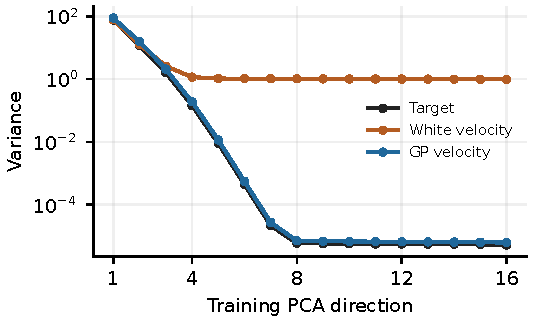
\includegraphics[width=\columnwidth]{geometry.pdf}
\caption{Training covariance spectra from the main experiment; held-out energy is reported separately in Table~\ref{tab:geometry}. Highly unequal variances explain why equality of raw directional errors is not a general accuracy target.}
\end{figure}

\clearpage
\section{Follow-up interventions and mechanism limits}
The following studies were designed after earlier outcomes were known. Their local protocols and hashes were frozen before scored training, but they are exploratory follow-ups rather than externally preregistered confirmations. They preserve every original result.

\subsection{The information-matched reference}
After history centering and scaling, conditioning on normalized history differs from conditioning on raw history. Integrating out the missing location and scale yields a generally non-Gaussian predictive mixture. In the no-floor idealization it has a Student-$t$ form with $L-1$ degrees of freedom; the implementation handles the normalization floor and numerically checks the correction.

The learned regression optimum is
\begin{equation}
 v^*(x,t,h)=\E[u\mid x_t=x,t,h].
\end{equation}
Consequently, independent-coupling velocity MSE includes conditional label variance even for the optimal field. A residual MSE floor cannot be equated to a failure to learn fine structure. The new reference matches the network's observed history, while retaining privileged knowledge of the synthetic population. The learned encoder may still discard information.

The oracle audit checks numerical quadrature, moments, finite differences, and independent derivations. Its derivative includes posterior mixture-weight changes. A raw unweighted residual-block Jacobian comparison favors S4, whereas conditional-input-covariance weighting reverses that ordering. Finite perturbation probes reproduce the sensitivity to weighting. These local errors are explanatory diagnostics, not proper forecast scores or a demonstrated causal explanation of optimization.

\paragraph{Loss weighting is a separate intervention.}
A controlled three-seed, identity-history study changes only directional loss weighting within its paired design. Raw-loss normalized residual MSE is 0.222 for MLP and 31.122 for S4; balanced loss gives 0.175 and 0.158. Raw residual error still favors MLP, and balancing raises PC1 error. The S4 target-PCA tail second-moment ratio changes from 597 to 0.585, correcting excess while undershooting the reference. This floor-sensitive tail effect does not establish improved meaningful curvature or forecast superiority. Full coordinate whitening differs from loss-only balancing; exact inputs and outputs are retained in temporal coordinates.

\subsection{A decoder constraint at horizon 64}
An exploratory long-window scan used $F=64$ with an MLP width of 56. For a velocity head $v=Wz+b$, let $P$ project orthogonally to the output column space. Then
\begin{equation}
 Pv=Pb,\qquad Px(1)=Px(0)+Pb.
\end{equation}
Thus the conditional source variance cannot change in that fixed subspace. There are at least eight such directions for the width-56 decoder, independent of training duration. Final LayerNorm can impose further local constraints. The main $F=16$ model has no corresponding width-below-horizon constraint.

A fresh capacity study uses three paired data/optimization replicates, $L=128,F=64,\ell=8$, white/GP sources, RBF and OU targets, and 36 fits. Each fit runs 12,000 updates; separately selected best-validation checkpoints at 6,000 and 12,000 are correlated budget observations, not 72 independent trainings. RBF controls are width-56/depth-3 MLP (73,960 parameters), width-65/depth-2 MLP (73,953), S4 (74,038), and larger width-72/depth-3 MLP (114,328). Width 65 clears the guaranteed final-LayerNorm rank cap below 64; numerical attenuation may persist.
\begin{table}[h]
\centering\small\begin{tabular}{lrrr}
\toprule
Source / head & $M_R$ & CRPS & $R/R_y$ \\
\midrule
gp / MLP56 & 0.7063 & 0.6287 & 0.989 \\
gp / MLP65 & 0.7063 & 0.6287 & 0.987 \\
gp / MLP72 & 0.7063 & 0.6296 & 0.988 \\
gp / S4 & 0.7058 & 0.6284 & 0.970 \\
white / MLP56 & 0.4644 & 0.6352 & 2.677 \\
white / MLP65 & 0.3546 & 0.6309 & 1.063 \\
white / MLP72 & 0.3423 & 0.6318 & 0.997 \\
white / S4 & 0.3262 & 0.6321 & 0.972 \\
\bottomrule
\end{tabular}

\caption{RBF capacity study at the 12,000-update budget; means over three fresh paired draws. Width/depth and larger-capacity controls have distinct interpretations.}\label{tab:capacity}
\end{table}

The parameter-matched width-65 MLP closes 79.4\% of the mean white-source residual gap between original MLP and S4; the larger same-depth control closes 88.4\%. Excess first-difference roughness largely disappears. This supports a consequential architectural confound in the old horizon-64 result. It does not show that widening removes every difference: S4 retains lower residual error, whereas CRPS ordering differs. Depth changes in the matched control, so its effect is interpreted jointly with the output invariant and the larger same-depth model.

GP-source residual errors are nearly equal across these heads. OU results further limit generalization from one kernel. Both the capacity setting and normalized ETTh1 extension lie outside the original rank-two geometry gate. They are robustness studies, not additional successful columns of the original assignment. A no-transport source is also scored for every capacity kernel/source/draw group, preventing inherited source smoothness from being mistaken for learned conditional forecasting.

\clearpage
\subsection{Normalization changes the ETTh1 head contrast}
ETTh1 uses only the OT channel, $L=48,F=24$, and chronological split endpoints 8,640/11,520/14,400. Windows are fully contained in their intervals; stride is 4 in training and 24 in validation/test. Global mean and standard deviation are fitted on training observations. All 118 test windows are scored with 64 members at Euler-64 in common train-standardized units.

Five pipelines separate global scaling, history centering, history scaling, both, and both with raw-unit-equivalent loss weighting. Additional GP-level controls remove or independently replace the constant source component. Across sources, heads, and three optimization seeds (71--73), this gives 84 fits. Best checkpoints within 2,000 and 6,000 updates are evaluated after training; these are not additional datasets.
\begin{table}[h]
\centering\small\begin{tabular}{lrrr}
\toprule
Pipeline & GP MLP & GP S4 & Ridge \\
\midrule
global & 0.2165 & 0.1748 & 0.1015 \\
center & 0.0982 & 0.0981 & 0.0973 \\
scale & 0.1179 & 0.1327 & 0.0983 \\
history & 0.0985 & 0.1005 & 0.0936 \\
history\_rawloss & 0.0992 & 0.1013 & 0.0943 \\
\bottomrule
\end{tabular}

\caption{ETTh1 fair CRPS at the 6,000-update budget. All pipelines are evaluated in the same units; smaller is better.}\label{tab:norm}
\end{table}

The GP-source MLP-minus-S4 point-estimate gap shrinks from 0.04168 under global scaling (0.21648 versus 0.17480) to 0.000139 with center-only normalization (0.09821 versus 0.09807). This does not establish equivalence. Scale-only GP instead favors MLP. There is no normalization-independent head winner. These interventions modify the entire conditioning/source/loss/selection pipeline and do not identify a unique internal cause.

A validation-tuned direct ridge baseline is retained; global ridge CRPS is 0.10148, already close to the centered flow results. Under history normalization, ridge CRPS is 0.09362 versus 0.09870 for white-source MLP and 0.09847 for GP-source MLP on the same 118 contexts. This prevents the head comparison from implying that flow training is necessary for this series. Similar CRPS can also conceal different interval widths and coverage. Training-defined scale strata contain 102 low-, 15 middle-, and one high-scale test histories; the last bin cannot support a reliable population statement.

This test period had already been inspected. Circular-block bootstrap intervals (block lengths 4 and 8) describe within-period sensitivity and serial dependence, not independent-series evidence or an untouched test. The two block lengths are sensitivity analyses, not two confirmations. No forecast score from this follow-up selects a new primary model.

\subsection{Conditional-mean supervision reduces some errors}
A 24-fit intervention returns to the original $L=32,F=16,\ell=8$ geometry with three fresh data draws, paired to seeds 81--83. Both source families and both heads are trained on the same precomputed 6,000-by-256 stream of interpolation inputs. The training target is either the ordinary label $u$ or the information-matched conditional mean $v^*$. Both modes select checkpoints using validation oracle discrepancy, so selection policy is controlled within this study but differs from the original experiment.

Conditional expectation preserves the population squared-loss optimum while removing conditional label variance. With a finite empirical history pool, it does not preserve every finite-sample paired-label objective. The intervention uses population knowledge unavailable in deployment; it measures the effect of conditional-mean supervision, not an implementable general forecasting method or optimizer noise in isolation.
\begin{table}[h]
\centering\footnotesize\begin{tabular}{lrrrr}
\toprule
Source / head & CRPS S & CRPS C & Gap S & Gap C \\
\midrule
white / MLP & 0.5073 & 0.4820 & 0.05967 & 0.04713 \\
white / S4 & 0.5060 & 0.4828 & 0.05177 & 0.04614 \\
gp / MLP & 0.4932 & 0.4785 & 0.01582 & 0.01314 \\
gp / S4 & 0.4923 & 0.4798 & 0.02466 & 0.02105 \\
\bottomrule
\end{tabular}

\caption{Means over three fresh paired draws. S: stochastic labels; C: conditional-mean labels. Gap is residual velocity discrepancy from the information-matched field, distinct from label MSE.}\label{tab:label}
\end{table}

Residual discrepancy improves in all 12 source/head/draw pairs. Forecast CRPS improves in 6/6 MLP pairs and 4/6 S4 pairs; neither head reaches the exact predictive reference. Eleven of 24 selected checkpoints occur at the final step, a warning against convergence claims. All 24 literal flags remain failures.

Full ensembles at Euler-128 are regenerated for every frozen checkpoint with the same 256 histories and 32 source draws; Euler-64 replay and independent arithmetic checks validate the comparison. Small numerical contrast reversals are recorded rather than promoted to substantive effects. Two resolutions cannot establish exact ODE solutions. The main label-study table retains its original Euler-64 results.

\clearpage
\section{Multivariate prediction and joint whitening}
\subsection{A common extension protocol}
We next examine jointly generated trajectories with three correlated synthetic GP channels, all seven ETTh1 variables \cite{informer}, and all eight Exchange variables \cite{lstnet}. The ETTh1 OT-only task supplies a one-channel anchor. These are archived exploratory experiments, re-summarized here without new training. They test transfer of the source/head comparison beyond the original geometry; the univariate rank-two gate is not imposed.

Each head receives the full history through an identity encoder and is trained for 2,000 updates, batch 128, with the same AdamW settings and three optimization seeds (31--33). Validation selects checkpoints every 250 updates. Widths target approximately 64,000 active parameters; the whitened MLP retains the reference MLP width. All scores use fixed training-only channel means and population standard deviations, with no per-window history normalization. Whitening fits a full joint $FC$-dimensional velocity PCA on training data, retains every coordinate with the declared floor, and maps predictions back before scoring. Its weighted validation objective is part of the intervention.

The synthetic process has $L=32,F=16$, channel equicorrelation 0.6, and 8,192/1,024/1,024 independent train/validation/test windows. ETTh1 uses $48\to24$ and the chronological boundaries specified above; Exchange uses $32\to16$ and 70/10/20\% chronological segments. Entire windows remain within a segment. Channel scaling and source cross-channel correlation are estimated from training data only.

The sources differ in temporal covariance while holding cross-channel covariance fixed: $I_F\otimes C_{\rm train}$ versus a unit-diagonal RBF kernel ($\ell=8$) $\otimes C_{\rm train}$, with 5\% correlation shrinkage toward identity. Thus ``white'' is temporally white, not independent across channels. A GP source for real targets is a modeling choice, not a claim that those targets are Gaussian processes.

\subsection{Forecast scores and direct baselines}
All cells use the same 64 selected test contexts, 32 members and Euler-64. Marginal fair CRPS averages all time/channel coordinates. Joint energy uses the full $FC$-vector and divides its Euclidean fair score by $\sqrt{FC}$. Both are lower-better; compare heads within a dataset. The scaled energy numbers do not share the scale of Table~\ref{tab:ensemble}.

\begin{table}[h]
\centering\footnotesize\begin{tabular}{lrrrr}
\toprule
Dataset (C) / source & MLP & S4 & Whiten. & Ridge \\
\midrule
GP (3) / W & 0.3288 & 0.3330 & 0.3439 & 0.1929 \\
GP (3) / G & 0.3328 & 0.3318 & 0.3095 & 0.1929 \\
ETTh1 OT (1) / W & 0.1422 & 0.1704 & 0.1284 & 0.0933 \\
ETTh1 OT (1) / G & 0.1950 & 0.1437 & 0.1321 & 0.0933 \\
ETTh1 (7) / W & 0.3621 & 0.4045 & 0.5268 & 0.2870 \\
ETTh1 (7) / G & 0.3750 & 0.4033 & 0.5298 & 0.2870 \\
Exchange (8) / W & 0.3137 & 0.3354 & 0.7071 & 0.0678 \\
Exchange (8) / G & 0.3852 & 0.4255 & 0.5640 & 0.0678 \\
\bottomrule
\end{tabular}

\caption{Extension fair CRPS, mean of three optimization seeds. W/G: temporally white/GP source; C: channels. Ridge includes whole-vector training-residual resampling and is shared across source rows.}\label{tab:multi_crps}
\end{table}

\begin{table}[h]
\centering\footnotesize\begin{tabular}{lrrrr}
\toprule
Dataset (C) / source & MLP & S4 & Whiten. & Ridge \\
\midrule
GP (3) / W & 0.4301 & 0.4357 & 0.4417 & 0.2806 \\
GP (3) / G & 0.4309 & 0.4297 & 0.4060 & 0.2806 \\
ETTh1 OT (1) / W & 0.1603 & 0.1904 & 0.1471 & 0.1104 \\
ETTh1 OT (1) / G & 0.2156 & 0.1639 & 0.1477 & 0.1104 \\
ETTh1 (7) / W & 0.4696 & 0.5483 & 0.6721 & 0.3984 \\
ETTh1 (7) / G & 0.5069 & 0.5420 & 0.6690 & 0.3984 \\
Exchange (8) / W & 0.3819 & 0.3934 & 0.8479 & 0.0926 \\
Exchange (8) / G & 0.4451 & 0.5048 & 0.6904 & 0.0926 \\
\bottomrule
\end{tabular}

\caption{Joint fair energy divided by $\sqrt{FC}$ on the same contexts and ensembles as Table~\ref{tab:multi_crps}. No cross-dataset ranking is implied.}\label{tab:multi_energy}
\end{table}

The GP-source S4 advantage on OT alone does not extend to the seven-channel ETTh1 average or Exchange: dense MLP has lower mean CRPS and joint energy than S4 in both multivariate real tasks and both sources. On the three-channel synthetic GP with a GP source, the head means are close. These fixed-budget observations do not establish an intrinsic architecture ranking.

Whitening improves mean CRPS in three of eight dataset/source cells: GP-source synthetic GP and both OT-only cells. It worsens both sources on seven-channel ETTh1 and eight-channel Exchange, and the joint energy comparison has the same directional pattern. For example, ETTh1/GP CRPS changes from 0.3750 to 0.5298, while Exchange/white changes from 0.3137 to 0.7071. The beneficial original univariate control therefore does not support a default whitening recommendation for real multivariate forecasting.

Ridge selects its penalty by validation MSE, then resamples complete in-sample training-residual vectors. It has lower mean CRPS and joint energy than every displayed neural cell on all four datasets. This is a practical baseline gap under the stated budget, not a guarantee that its residual uncertainty is calibrated under shift. Separate Elastic Net and other neural controls remain in the archived analyses.

A matched OT rescore aligns the same timestamps, OT targets and scaler: seven of eight joint head/source cells have higher mean OT CRPS than their univariate counterpart; the sole small reversal is white-source U-Net, with uncertainty spanning zero. This does not show that extra variables lack information. Output dimension, conditioning, source covariance, widths and optimization burden change together at similar total capacity. Nor is this a pure dimension intervention against the original study, which uses different normalization and training duration. Real-period block intervals remain exploratory and conditional, without multiplicity adjustment.

\clearpage
\section{What trajectory diagnostics add}
\subsection{Frozen ensembles and declared post-hoc scope}
Mean adjacent jumps are a single moment of a trajectory distribution. To test whether their apparent agreement hides finer discrepancies, we re-score 39 frozen forecast ensembles: 15 main GP-source checkpoints, 12 RBF/white capacity checkpoints, and 12 GP-source label-noise checkpoints. There is no new model fit, model selection, source draw, or generated forecast. Input hashes bind this analysis to existing arrays.

The canonical estimator uses an ensemble tensor $X\in\R^{N\times M\times F}$ and target $Y\in\R^{N\times F}$. A context is the observation unit. Main evaluation has $N=256,M=64$; the two follow-ups have $N=256,M=32$. Full 1,024-path roughness cohorts are stored in a separate namespace and never substituted for the proper-score cohort.

For $k\in\{1,2\}$,
\begin{equation}
 R_k(X)=\E_{h,m}\frac{1}{F-k}\sum_{i=1}^{F-k}|\Delta^k X_{hmi}|.
\end{equation}
Ratios divide pooled generated means by pooled target means. $R_2$ measures second differences; neither roughness ratio is a proper score or a new success gate. A ratio near one is moment agreement, not proof of calibrated trajectory dependence.

\subsection{Dependence-sensitive variogram score}
For $p=0.5$, let $a_{ij}=|y_i-y_j|^p$, $z_{mij}=|X_{mi}-X_{mj}|^p$, and normalized weights $w_{ij}\propto1/(j-i)$ over $i<j$. The plug-in score is
\begin{equation}
 \widehat{\mathrm{VS}}=\sum_{i<j}w_{ij}\left(a_{ij}-\bar z_{ij}\right)^2.
\end{equation}
Following fair ensemble scoring, we also report
\begin{equation}
 \widehat{\mathrm{VS}}_{\rm fair}=\widehat{\mathrm{VS}}-\sum_{i<j}w_{ij}\frac{s^2(z_{ij})}{M},
\end{equation}
using sample variance with $M-1$ denominator. This removes ensemble estimation variance for the population variogram functional under conditionally iid members. A fair estimate can be negative and is not clipped. The score is dependence-sensitive but does not identify the entire joint law or uniquely determine absolute level \cite{scheuerer,fair}.

\begin{table}[h]
\centering\footnotesize\begin{tabular}{lrrrr}
\toprule
Head & $R_1/R_{1y}$ & $R_2/R_{2y}$ & VS plug-in & VS fair \\
\midrule
mlp & 1.007 & 0.988 & 0.07310 & 0.07195 \\
s4 & 1.032 & 1.628 & 0.07106 & 0.06989 \\
whitened\_mlp & 1.005 & 0.990 & 0.06977 & 0.06866 \\
\bottomrule
\end{tabular}

\caption{Post-hoc main ensembles, using the 256-context cohort. All rows use identical observed targets. VS is lower-better; roughness ratios have no ordering interpretation beyond agreement with the reference moment.}\label{tab:trajectory}
\end{table}

Main S4 has $R_1$ ratio 1.032 but $R_2$ ratio 1.628. MLP and whitened MLP have $R_2$ ratios 0.988 and 0.990. Thus near-correct first differences can coexist with excess second differences. This is a specific diagnostic failure of $R_1$; it does not negate S4's forecast score values.

Whitened MLP minus raw MLP fair VS is $-0.003296$ with conditional paired-history 95\% interval $[-0.005310,-0.001420]$, and all five seedwise differences are negative. S4 minus MLP is $-0.002066$ with interval $[-0.004371,0.000020]$ and mixed seedwise signs. The former is evidence for this chosen exploratory functional on fixed models, not a retrospective proper-score winner. Metrics, contrasts, and follow-up choices were not multiplicity adjusted.

In RBF/white capacity ensembles, original MLP $R_2$ ratio is 19.09, falling to 1.687 and 1.602 for rank-cleared and wider controls; S4 is 1.002. Their fair VS values fall from 0.11117 to approximately 0.0923--0.0925, with improvements in all three paired replicates. Removing an output-space constraint matters to trajectory structure, even when marginal CRPS changes little. Across the three label-noise draws, proper scores and VS still do not give a consistent S4-versus-MLP advantage.

\begin{figure}[h]
\centering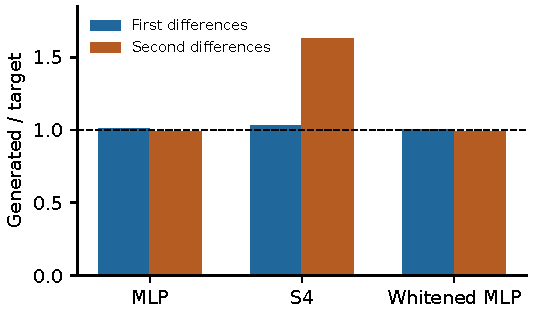
\includegraphics[width=\columnwidth]{roughness.pdf}
\caption{Main frozen ensembles: first- and second-difference ratios summarize distinct moments. The dashed line denotes target-moment agreement, not a proper-score optimum or success threshold.}
\end{figure}

\clearpage
\section{Limitations, reproducibility, and conclusion}
\subsection{Limits of the claims}
The primary data are one GP draw with a smooth univariate geometry. Its five seeds measure optimization variability, not data-generation uncertainty. Follow-ups use three paired data/optimization replicates, so dataset and initialization effects cannot be separated. RBF and OU intentionally share random-number seeds. The normalization intervention uses only ETTh1 OT, while the separate global-scaling extension includes seven-channel ETTh1 and eight-channel Exchange. Each real dataset still supplies one fixed chronological test segment; these experiments are not a broad benchmark of real-world forecasting.

Our small S4 implementation is mathematically checked against independent complex-reference kernels and gradients, but it has reduced state size and a short-patch implementation. Our MLP copies a released architectural pattern without pretrained weights or the complete original objective. Neither model has broad hyperparameter optimization. Conditioning is also unmatched: AdaLN modulates the MLP, whereas S4 uses additive/bias conditioning. A matched AdaLN-S4 control and a broad learning-rate-by-conditioning sweep remain open. S4 learns internal step sizes $\Delta$, initialized log-uniformly over $[0.001,0.1]$; these are initialization bounds, not enforced bounds during training. No initialization-range ablation was performed. Internal S4 discretization, Euler transport step count, and Fourier flow-time embedding are distinct choices; a solver check does not test the other two. Time-conditioning, whitening-floor and shrinkage ablations also remain open. Shared encoder initialization does not imply identical learned representations. The equal-count capacity control changes depth; the same-depth wider model changes parameter count. These controls narrow interpretation without isolating all architecture factors.

Raw pairwise velocity error includes conditional regression noise; source families have different labels and different noise floors. A privileged reference sees more history information, while the matched reference knows the generating population. Neither is an ordinary deployable baseline. GP normalization changes the target law and the physical meaning of independent source coordinates. Whitening and balancing depend on a floor affecting ten directions; neither is a neutral unit conversion of the learning problem.

Optimization and numerical errors remain. Warm restarts improve validation losses, and some new fits select the final checkpoint. Fixed-step Euler can distort conditional covariance even when mean roughness appears correct. Local Jacobian norms depend strongly on weighting and cannot establish forecast quality. Two solver resolutions check sensitivity, not convergence to an exact transport.

The fixed criterion was operationalized before scored fits, but the geometry was informed by a pilot. Later questions arose from observed results and the ETTh1 period was reused. All exploratory analyses are labeled; no retrospective rule, metric, or favorable subset replaces the original outcome. Bootstrap intervals are descriptive and conditional on the specified evaluation units, without multiplicity adjustment. A score interval spanning zero is not an equivalence test.

\subsection{Audit and computational record}
Core implementation is in \src{fm_stress/data.py}, \src{models.py}, \src{experiment.py}, and \src{metrics.py} (all latter paths relative to \src{fm_stress/}). Independent array reconstruction and source/configuration hashes check normalization, RNG pairing, train-fitted PCA, checkpoint selection, and metric arithmetic. Follow-up audits replay old checkpoints and independently reconstruct forecast scores; architectural loading is reused where required. ``Independent'' here describes separate implementations and agent reviews, not a claim of independent human replication.

The main runs report MPS with PyTorch 2.14.1 on an Apple M3 Pro environment. Their stored run-duration fields sum to \MainLoggedSeconds\ seconds. This is the sum of a specific logged field for 25 runs, not a comprehensive end-to-end project compute budget. The broader archived extension contains 96 fits; the sparse/whitening archive adds 264 main fits and 24 dictionary controls (288 additional fits), reusing the 96 references. The compact multivariate tables select 24 source/head/dataset cells, or 72 existing checkpoints. The revision performs no new training and does not claim those archive counts are all newly analyzed fits. New studies ran on MPS, whereas historical long-window scans included CUDA and replay used CPU. Concurrent processes, preparation, oracle construction, numerical audits, and omitted exploratory studies preclude a defensible total dedicated-device-hour or architecture-speed claim. The canonical evidence file preserves raw timing metadata with scope notes.

Every paper table is generated from recorded JSON by \src{scripts/build_final_paper.py}; \src{output/final-paper/evidence.json} preserves full-precision values and consumed-source SHA256 hashes. Appendix~\ref{app:reproduce} identifies configurations, seeds, and exact scripts. The frozen delivery revision and package checks are recorded in \src{FINAL_PACKAGE.json} and \src{docs/final_package.md}; a source hash manifest is more precise than claiming the final paper itself existed at the original experiment revision.

\subsection{Conclusion}
This controlled experiment does not support switching to the tested S4 head on the basis of a smooth GP source. The retained formal criterion is inconclusive, and fresh-history proper scores do not establish head superiority. Whitening lowers primary velocity errors but worsens both real multivariate tasks in the joint extension, where direct ridge forecasts retain lower scores. Capacity controls expose a consequential long-horizon decoder constraint; normalization changes the real-series ranking; conditional-mean supervision improves some errors without solving forecasting. First-difference roughness alone misses excess second differences. Future comparisons should prospectively define forecast and trajectory estimands, clear avoidable decoder constraints, and test full pipelines across independent datasets and budgets.

\paragraph{Author contributions.}

\textbf{Egor Serov.} Implemented the MLP and shared training pipeline; organized controlled source-by-head comparisons; investigated decoder width and model capacity; and prepared the reproducible experimental protocol.

\textbf{Kirill Frolov.} Prepared synthetic data and PCA analyses; examined the original evaluation criteria and added R2 and Variogram Score diagnostics; analyzed archived forecasts, checked numerical consistency, and consolidated the final materials.

\textbf{Daniil Koblov.} Implemented and validated S4 and structured forecasting models; adapted them to joint multivariate prediction; compared source distributions and investigated how findings transfer from synthetic to real data.

\textbf{Vasilii Lyamin.} Studied whitening and normalization; analyzed head Jacobians, kernel settings, and result sensitivity; investigated mechanisms behind model differences, visualized diagnostics, and formulated the limitations of the conclusions.


\paragraph{AI assistance and responsibility.}
AI coding agents assisted with implementation, numerical analysis, audit scripts, drafting, and artifact preparation. Separate agent checks and executable tests improve traceability but are not independent human validation. The named authors remain responsible for verifying the evidence, understanding the methods, confirming the submission, and presenting the work.

\begin{thebibliography}{9}\small
\bibitem{lipman} Y. Lipman, R. T. Q. Chen, H. Ben-Hamu, M. Nickel, and M. Le. Flow Matching for Generative Modeling. ICLR, 2023. \url{https://arxiv.org/abs/2210.02747v2}.
\bibitem{sundial} Y. Liu et al. Sundial: A Family of Highly Capable Time Series Foundation Models. 2025. Inspected manuscript v2. \url{https://arxiv.org/abs/2502.00816v2}.
\bibitem{tsflow} M. Kollovieh, M. Lienen, D. L\"udke, L. Schwinn, and S. G\"unnemann. Flow Matching with Gaussian Process Priors for Probabilistic Time Series Forecasting. 2025. \url{https://arxiv.org/abs/2410.03024v2}.
\bibitem{s4} A. Gu, K. Goel, and C. R\'e. Efficiently Modeling Long Sequences with Structured State Spaces. ICLR, 2022. \url{https://arxiv.org/abs/2111.00396v3}.
\bibitem{scheuerer} M. Scheuerer and T. M. Hamill. Variogram-based proper scoring rules for probabilistic forecasts of multivariate quantities. Monthly Weather Review, 143:1321--1334, 2015. \url{https://doi.org/10.1175/MWR-D-14-00269.1}.
\bibitem{fair} C. A. T. Ferro. Fair scores for ensemble forecasts. Quarterly Journal of the Royal Meteorological Society, 140:1917--1923, 2014. \url{https://doi.org/10.1002/qj.2270}.
\bibitem{informer} H. Zhou et al. Informer: Beyond Efficient Transformer for Long Sequence Time-Series Forecasting. AAAI, 2021. \url{https://arxiv.org/abs/2012.07436v3}.
\bibitem{lstnet} G. Lai, W.-C. Chang, Y. Yang, and H. Liu. Modeling Long- and Short-Term Temporal Patterns with Deep Neural Networks. SIGIR, 2018. \url{https://arxiv.org/abs/1703.07015v3}.
\end{thebibliography}

\appendix
\setlength{\parskip}{0pt}
\section{Reproduction and evidence map}\label{app:reproduce}
\subsection{Environment and release boundaries}
Use Python 3.12 and \src{requirements-lock.txt}. Environment/provenance manifests identify the actual runs. MPS training requires Metal access; CPU replay and metric-only checks do not. Rebuilding tables requires no retraining.

\begin{verbatim}
python3 -m venv .venv
.venv/bin/python -m pip install \
  -r requirements-lock.txt
.venv/bin/python -m pytest -q
\end{verbatim}
Historical/supplementary archives do not enlarge this paper's estimand. Interrupted workers (including capacity pre-audit), smokes, pilots, repeated budget checkpoints and numerical replay are excluded from independent-fit counts.

\subsection{Original experiment}
The complete configuration is \src{configs/main.json}; data seed 27041; optimization seeds 0--4; $L=32,F=16,\ell=8$; 6,000 updates; Euler-64. Run from the repository root:
\begin{verbatim}
python -m fm_stress.experiment geometry \
 --config configs/main.json \
 --output results/main
python -m fm_stress.experiment train \
 --config configs/main.json \
 --output results/main --device mps
python -m fm_stress.experiment oracle \
 --config configs/main.json \
 --output results/main
python -m fm_stress.analyze \
 --results results/main \
 --output output/analysis \
 --require-complete
\end{verbatim}
Artifacts: \src{results/main/}. Criterion: \src{docs/protocol.md}. Adaptations and source revisions: \src{docs/model_provenance.md}. The Sundial head is pinned to HF revision \src{3212e42564493f520593e5414af4367fc4b49226}; S4 source revision is\par\noindent{\footnotesize\src{e757cef57d89e448c413de7325ed5601aceaac13}}. References/licenses: \src{vendor/}.

\subsection{Forecast and matched-reference evaluation}
\src{configs/ensemble_evaluation.json}, \src{fm_stress/ensemble_evaluation.py}, and \src{fm_stress/analyze_ensemble.py} define the fresh 256-context, 64-member main evaluation. Data/source/reference seeds are 87041/88041/89041. The paired-context bootstrap uses seed 90041 and 10,000 draws. Canonical outputs are \src{results/ensemble-evaluation/summary.json} and archived per-context arrays.

Matched oracle: \src{fm_stress/normalized_history_oracle.py}; runs/convergence checks: \src{results/followup-oracle/}; conditioning protocol: \src{docs/followup_oracle_protocol.md}. Covariance-weighted probes are post-hoc.

\subsection{Follow-up training and selection}
Capacity: \src{configs/followup_capacity.json}, \src{fm_stress/followup_capacity.py}, \src{scripts/analyze_followup_capacity.py}. Data seeds 607041/707041/807041 pair with optimization seeds 61/62/63. The canonical summary is \src{output/followup-capacity/summary.json}; all 36 fits and both budget records are retained. \src{scripts/audit_followup_decoder_span.py} and \src{scripts/check_followup_capacity.py} check the decoder identities and results.

Normalization: \src{configs/followup_normalization.json}, \src{fm_stress/followup_normalization.py}, and \src{scripts/analyze_followup_normalization.py}. Seeds 71--73 share the chronological ETTh1 split. Train-only scaling, full interval containment, 118 test contexts, and matched output units are checked independently. Final summary: \src{output/followup-normalization/summary.json}; review: \src{docs/followup_normalization_final_review.md}.

Label variance: \src{configs/followup_label_noise.json}, \src{fm_stress/followup_label_noise.py}, and \src{scripts/analyze_followup_label_noise.py}. Data seeds 917041/1017041/1117041 pair with seeds 81/82/83. The 24-fit summary is \src{output/followup-label-noise/summary.json}. Full solver re-scoring uses \src{scripts/study_followup_label_solver.py}; original checkpoint/source hashes are checked before and after generation. The original 64-step study remains distinct from \src{results/followup-label-solver/}.

\subsection{Multivariate and joint-whitening extension}
\src{configs/extension.json} and \src{configs/sparse_extension.json} fix the common four-dataset protocol. Training and scoring implementations are \src{fm_stress/extended_experiment.py}, \src{fm_stress/sparse_experiment.py}, \src{fm_stress/extended_data.py}, and \src{fm_stress/extended_metrics.py}. Canonical aggregation is in \src{output/extension-analysis/summary.json} and \src{output/sparse-analysis/summary.json}; no new model or ensemble is generated for the present paper revision.

\begin{verbatim}
python scripts/fetch_extension_data.py
python -m fm_stress.extended_experiment \
 --device mps
python scripts/check_extension.py
python -m fm_stress.analyze_extension
python -m fm_stress.sparse_experiment \
 --device mps
python scripts/check_sparse_extension.py
python -m fm_stress.analyze_sparse
python scripts/check_sparse_analysis.py
\end{verbatim}
The separate 24-fit dictionary control, \src{configs/sparse_fullrank_dictionary.json}, is excluded from the 72 displayed checkpoints. Full pipeline: \src{scripts/run_sparse.sh}. Raw-data revisions/hashes: \src{data/real/manifest.json}; raw files are excluded from Git. ETTh1/Exchange come from the authors' ETDataset/multivariate-time-series-data repositories; source terms: \src{docs/extension_protocol.md}.

The 96-fit run replay is \src{results/extension/independent_verification.json}. Independent aggregation checks are \src{results/diagnostics/extension_analysis_verification.json} and \src{results/diagnostics/sparse_analysis_verification.json}; the latter checks 264 new plus 96 frozen reference records. \src{results/diagnostics/dictionary_analysis_verification.json} separately audits the structural supplement. These audit arithmetic/provenance, not interval coverage. Seeds 31--33 share datasets/periods. Whitening retains reference width and full joint PCA with inverse mapping and the stated floor.

\subsection{Additional exploratory source control}
A separate covariance-mixture control uses $C_\epsilon=0.5I+0.5K$ (unit diagonal), two independent data draws, and three optimization seeds per draw. Recorded fair CRPS is 0.49196 for MLP, 0.49076 for S4, and 0.53308 for whitened MLP. This is not an exact-covariance conditional reference and does not establish that an intermediate prior is universally preferable. The canonical configuration and results remain in \src{configs/prior_mixture.json} and \src{output/prior-mixture/}; this exploratory control does not replace the main source families.

\subsection{New trajectory analysis and paper build}
\src{fm_stress/trajectory_metrics.py} implements the frozen-array metrics; \src{docs/trajectory_metrics.md} defines their uncertainty units. \src{results/trajectory-metrics/summary.json} and adjacent arrays preserve canonical scores and input hashes. Rebuild scoring and paper assets with:

\begin{verbatim}
python scripts/evaluate_trajectory_metrics.py
python scripts/build_final_paper.py
\end{verbatim}
\end{document}
